\documentclass{article}
\usepackage{v-test-paper}
\title{\textsc{JEE Advanced 2022 Paper-I\\Physics}}
\date{}
\begin{document}
\maketitle


\begin{enumerate}
    \item Two spherical stars \(A\) and \(B\) have densities \(\rho_A\) and \(\rho_B\), respectively. \(A\) and \(B\) have the same radius, and their masses \(M_A\) and \(M_B\) are related by \(M_B = 2M_A\). Due to an interaction process, star \(A\) loses some of its mass, so that its radius is halved, while its spherical shape is retained, and its density remains \( \rho_A \). The entire mass lost by \(A\) is deposited as a thick spherical shell on \(B\) with the density of the shell being \( \rho_B \). If \( v_{A} \) and \( v_{B} \) are the escape velocities from \(A\) and \(B\) after the interaction process, the ratio \( \frac{v_{B}}{v_{A}} = \frac{10n}{\sqrt{15}} \). The value of \(n\) is \_\_\_\_\_.

    \item The minimum kinetic energy needed by an alpha particle to cause the nuclear reaction \[ ^{16}_{7}N + ^{4}_{2}He \rightarrow ^{1}_{1}H + ^{19}_{8}O + n \] in laboratory frame is in \(MeV\). Assume that \(^{16}N\) is at rest in the laboratory frame. The masses of \(^{16}N\), \(^{4}He\), \(^{19}O\) and \(n\) can be taken to be 16.006 u, 4.003 u, 19.008 u and 1.009 u, respectively, where 1 u = 930 \(MeV/c^2\). The value of \(n\) is \_\_\_\_\_.

    \item In the following circuit \(C_1 = 12 \mu F\), \(C_2 = C_3 = 4 \mu F\) and \(C_4 = C_5 = 2 \mu F\). The charge stored in \(C_3\) is \_\_\_\_ \(\mu C\).
    \begin{center}
        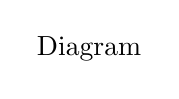
\begin{tikzpicture}
            \node {Diagram};
        \end{tikzpicture}
    \end{center}

    \item A rod of length 2 cm makes an angle \(\frac{2\pi}{3}\) rad with the principal axis of a thin convex lens. The lens has a focal length of 10 cm and is placed at a distance of \(\frac{40}{3}\) cm from the object as shown in the figure. The height of the image is \(\frac{30 \sqrt{3}}{13}\) cm and the angle made by it with respect to the principal axis is \(\frac{\alpha}{n}\) rad, where \(n\) is \_\_\_\_\_.
    \begin{center}
        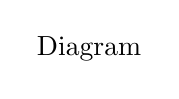
\begin{tikzpicture}
            \node {Diagram};
        \end{tikzpicture}
    \end{center}

    \item At time $t = 0$, a disk of radius $1$ m starts to roll without slipping on a horizontal plane with an angular acceleration of $\alpha = 2 \text{ rad s}^{-2}$. A small stone is stuck to the disk. At $t = 0$, it is at the contact point of the disk and the plane. Later, at time $t = \sqrt{\frac{\pi}{\alpha}}$, the stone detaches itself and flies off tangentially from the disk. The maximum height (in m) reached by the stone measured from the plane is $\frac{1}{2} \pi + \frac{x}{10}$. The value of $x$ is \underline{\hspace{3cm}}. [Take $g = 10$ m s$^{-2}$.]

    \item A solid sphere of mass $1$ kg and radius $1$ m rolls without slipping on a fixed inclined plane with an angle of inclination $\theta = 30^\circ$ from the horizontal. Two forces of magnitude $1$ N each, parallel to the incline, act on the sphere, both at the horizontal 0.5 m from the center of the sphere, as shown in the figure. The acceleration of the sphere down the plane is \underline{\hspace{3cm}} m s$^{-2}$. [Take $g = 10$ m s$^{-2}$.]
    
    \begin{center}
        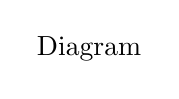
\begin{tikzpicture}
            \node {Diagram};
        \end{tikzpicture}
    \end{center}
	
    \item Consider an LC circuit, with inductance $L = 0.1$ H and capacitance $C = 10^{-3}$F, kept on a plane. The area of the circuit is $1$ m$^2$. It is placed in a constant magnetic field of strength $B_0$ which is perpendicular to the plane of the circuit. At time $t = 0$, the magnetic field strength starts increasing linearly as $B = B_0 + \beta t$ with $\beta = 0.04$ T s$^{-1}$. The maximum magnitude of the current in the circuit is \underline{\hspace{3cm}} mA.

    \item A projectile is fired from horizontal ground with speed $v$ and projection angle $\theta$. When the acceleration due to gravity is $g$, the range of the projectile is $d$. If at the highest point in its trajectory, the projectile enters a different region where the effective acceleration due to gravity is $g' = \frac{g}{0.81}$, then the new range is $d' = n d$. The value of $n$ is \underline{\hspace{3cm}}.

    \item A medium having dielectric constant  $K > 1$ fills the space between the plates of a parallel plate capacitor. The plates have large area, and the distance between them is $d$. The capacitor is connected to a battery of voltage $V$, as shown in Figure (a). Now, both the plates are moved by a distance of $\frac{d}{2}$ from their original positions, as shown in Figure (b).
    \begin{center}
        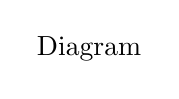
\begin{tikzpicture}
            \node {Diagram};
        \end{tikzpicture}
    \end{center}
    In the process of going from the configuration depicted in Figure (a) to that in Figure (b), which of the following statement(s) is(are) correct?
    
        \begin{tasks}(1)
            	\task The electric field inside the dielectric material is reduced by a factor of 2K.
            	\task The capacitance is decreased by a factor of $\frac{1}{K+1}$.
            	\task The voltage between the capacitor plates is increased by a factor of (K + 1).
            	\task The work done in the process DOES NOT depend on the presence of the dielectric material.
        \end{tasks}

    \item The figure shows a circuit having eight resistances of \(1 \Omega\) each, labelled \(R_1\) to \(R_8\), and two ideal batteries with voltages \(\epsilon_1 = 12 \text{ V}\) and \(\epsilon_2 = 6 \text{ V}\). 
    \begin{center}
        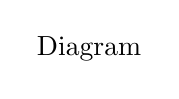
\begin{tikzpicture}
            \node {Diagram};
        \end{tikzpicture}
    \end{center}
    Which of the following statement(s) is(are) correct?
        \begin{tasks}(1)
            \task The magnitude of current flowing through \(R_1\) is \(7.2 \text{ A}\).
            \task The magnitude of current flowing through \(R_2\) is \(1.2 \text{ A}\).
            \task The magnitude of current flowing through \(R_3\) is \(4.8 \text{ A}\).
            \task The magnitude of current flowing through \(R_5\) is \(2.4 \text{ A}\).
        \end{tasks}


    \item An ideal gas of density \( \rho = 0.2 \, \text{kg m}^{-3} \) enters a chimney of height \( h \) at the rate of \( \alpha = 0.8 \, \text{kgs}^{-1} \) from its lower end, and escapes through the upper end as shown in the figure. The cross-sectional area of the lower end is \( A_1 = 0.1 \, \text{m}^2 \) and the upper end is \( A_2 = 0.4 \, \text{m}^2 \). The pressure and the temperature of the gas at the lower end are 600 Pa and 300 K, respectively, while its temperature at the upper end is 150 K. The chimney is heat insulated so that the gas undergoes adiabatic expansion. Take \( g = 10 \, \text{ms}^{-2} \) and the ratio of specific heats of the gas \( \gamma = 2 \). Ignore atmospheric pressure.

\begin{center}
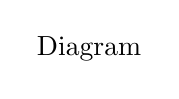
\begin{tikzpicture}
\node {Diagram};
\end{tikzpicture}
\end{center}

Which of the following statement(s) is(are) correct?

\begin{tasks}(1)
\task The pressure of the gas at the upper end of the chimney is 300 Pa.
\task The velocity of the gas at the lower end of the chimney is \( 40 \, \text{ms}^{-1} \) and at the upper end is \( 20 \, \text{ms}^{-1} \).
\task The height of the chimney is 590 m.
\task The density of the gas at the upper end is \( 0.05 \, \text{kg m}^{-3} \).
\end{tasks}

    \item Three plane mirrors form an equilateral triangle with each side of length \( L \). There is a small hole at a distance \( l > 0 \) from one of the corners as shown in the figure. A ray of light is passed through the hole at an angle \( \theta \) and can only come out through the same hole. The cross section of the mirror configuration and the ray of light lie on the same plane.

    \begin{center}
        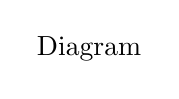
\begin{tikzpicture}
            \node {Diagram};
        \end{tikzpicture}
    \end{center}

    Which of the following statement(s) is(are) correct?

    \begin{tasks}(1)
    \task The ray of light will come out for \( \theta = 30^\circ \), for \( 0 < l < L \).
    \task There is an angle for \( l = \frac{L}{2} \) at which the ray of light will come out after two reflections.
    \task The ray of light will NEVER come out for \( \theta = 60^\circ \), and \( l = \frac{L}{3} \).
    \task The ray of light will come out for \( \theta = 60^\circ \), and \( 0 < l < \frac{L}{2} \) after six reflections.
    \end{tasks}

    \item Six charges are placed around a regular hexagon of side length $a$ as shown in the figure. Five of them have charge $q$, and the remaining one has charge $x$. The perpendicular from each charge to the nearest hexagon side passes through the center $O$ of the hexagon and is bisected by the side.
    \begin{center}
        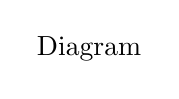
\begin{tikzpicture}
            \node {Diagram};
        \end{tikzpicture}
    \end{center} 
    Which of the following statement(s) is(are) correct in SI units?
        \begin{tasks}(1)
            	\task When $x = q$, the magnitude of the electric field at $O$ is zero.
            	\task When $x = -q$, the magnitude of the electric field at $O$ is $\frac{q}{6\pi \varepsilon_0 a^2}$.
            	\task When $x = 2q$, the potential at $O$ is $\frac{7q}{4\pi\varepsilon_0 a}$.
            	\task When $x = -3q$, the potential at $O$ is $-\frac{3q}{4\pi\varepsilon_0 a}$.
        \end{tasks}

    \item The binding energy of nucleons in a nucleus can be affected by the pairwise Coulomb repulsion. Assume that all nucleons are uniformly distributed inside the nucleus. Let the binding energy of a proton be $E_b^p$ and the binding energy of a neutron be $E_b^n$ in the nucleus.
    
    Which of the following statement(s) is(are) correct?
        \begin{tasks}(1)
            	\task $E_b^p - E_b^n$ is proportional to $Z(Z - 1)$ where $Z$ is the atomic number of the nucleus.
            	\task $E_b^p - E_b^n$ is proportional to $A^{-1/3}$ where $A$ is the mass number of the nucleus.
            	\task $E_b^p - E_b^n$ is positive.
            	\task $E_b^p$ increases if the nucleus undergoes a beta decay emitting a positron.
        \end{tasks}

  \item A small circular loop of area $A$ and resistance $R$ is fixed on a horizontal $xy$-plane with the center of the loop always on the axis of a long solenoid. The solenoid has $n$ turns per unit length and carries current $I$ counterclockwise as shown in the figure. The magnetic field due to the solenoid is in $\hat{i}$ direction. List-I gives time dependences of $\hat{i}$ in terms of a constant angular frequency $\omega$. List-II gives the torques experienced by the circular loop at time $t = \frac{\pi}{\omega}$.

  Let \(\alpha = \frac{A\mu_0^2 n^2 I^2}{2R}\).

    \begin{center}
        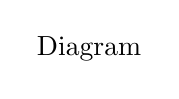
\begin{tikzpicture}
            \node {Diagram};
        \end{tikzpicture}
    \end{center}

\begin{center}
    \renewcommand{\arraystretch}{2}
    \begin{table}[h]
        \centering
        \begin{tabular}{p{0.25cm}p{8cm}|p{0.25cm}p{5cm}}
        \hline
        & Column I & & Column II \\
        \hline
        (I) & \( \frac{1}{\sqrt{2}} (\sin \omega t + \cos \omega t) \) & (P) & 0 \\
        (II) & \( \frac{1}{\sqrt{2}} (\sin \omega t + \cos \omega t) \) & (Q) & \( -\frac{\alpha}{4} \) \\
        (III) & \( \frac{1}{\sqrt{2}} (\sin \omega t + \cos \omega t) \) & (R) & \( \frac{3\alpha}{4} \) \\
        (IV) & \( \frac{1}{\sqrt{2}} (\cos \omega t + \sin \omega t) \) & (S) & \( \frac{3\alpha}{4} \) \\
        & & (T) & \( -\frac{3\alpha}{4} \) \\
        \hline
        \end{tabular}
    \end{table}
\end{center}


Which one of the following options is correct?

\begin{tasks}(2)
    \task (I) $\rightarrow$ (Q), (II) $\rightarrow$ (P), (III) $\rightarrow$ (S), (IV) $\rightarrow$ (T)
    \task (I) $\rightarrow$ (S), (II) $\rightarrow$ (T), (III) $\rightarrow$ (Q), (IV) $\rightarrow$ (P)
    \task (I) $\rightarrow$ (Q), (II) $\rightarrow$ (P), (III) $\rightarrow$ (S), (IV) $\rightarrow$ (R)
    \task (I) $\rightarrow$ (T), (II) $\rightarrow$ (Q), (III) $\rightarrow$ (P), (IV) $\rightarrow$ (R)
\end{tasks}





\item List I describes four systems, each with two particles $A$ and $B$ in relative motion as shown in figures. List II gives possible magnitudes of their relative velocities (in $\dfrac{m}{s}$) at time $t = \dfrac{\pi}{3}$.

\begin{center}
\renewcommand{\arraystretch}{1.5}
\begin{tabular}{p{0.5cm}p{10cm}|p{0.5cm}p{3cm}}
\hline
 & List-I & & List-II \\
\hline
(I) & $A$ and $B$ are moving on a horizontal circle of radius $1 m$ with uniform angular speed $\omega = 1 rad s^{-1}$. The initial angular positions of $A$ and $B$ at time $t = 0$ are $\theta = 0$ and $\theta = \frac{\pi}{2}$, respectively. 
& (P) & $\sqrt{3+1} \div 2$ \\
\hline
(II) & Projectiles $A$ and $B$ are fired (in the same vertical plane) at $t = 0$ and $t = 0.1 s$ respectively, with the same speed $v = \sqrt{\frac{5\pi}{2}} ms^{-1}$ and at $45^\circ$ from the horizontal plane. The initial separation between $A$ and $B$ is large enough so that they do not collide. ($g = 10 ms^{-2}$). 
& (Q) & $\frac{\sqrt{3-1}}{\sqrt{2}}$ \\
\hline
(III) & Two harmonic oscillators $A$ and $B$ moving in the $x$ direction according to $x_A = x_0 \sin \frac{t}{t_0}$ and $x_B = x_0 \sin(\frac{t}{t_0} + \frac{\pi}{2})$ respectively, starting from $t = 0$. Take $x_0 = 1m, t_0 = 1s$.
& (R) & $\sqrt{10}$ \\
\hline
(IV) & Particle $A$ is rotating in a horizontal circular path of radius $1 m$ on the $xy$ plane, with constant angular speed $\omega = 1 rad s^{-1}$. Particle $B$ is moving up at a constant speed $3 m s^{-1}$ in the vertical direction as shown in the figure. (Ignore gravity.)
& (S) & $\sqrt{2}$ \\
\hline
 & 
& (T) & $\sqrt{25\pi^2 + 1}$ \\
\hline
\end{tabular}
\end{center}

Which one of the following options is correct?

\begin{tasks}(2)
    \task(I) $\rightarrow$ R, (II) $\rightarrow$ T, (III) $\rightarrow$ P, (IV) $\rightarrow$ S
    \task(I) $\rightarrow$ S, (II) $\rightarrow$ P, (III) $\rightarrow$ Q, (IV) $\rightarrow$ R
    \task(I) $\rightarrow$ S, (II) $\rightarrow$ T, (III) $\rightarrow$ P, (IV) $\rightarrow$ R
    \task(I) $\rightarrow$ T, (II) $\rightarrow$ P, (III) $\rightarrow$ R, (IV) $\rightarrow$ S
\end{tasks}




\item List I describes thermodynamic processes in four different systems. List II gives the magnitudes (either exactly or as a close approximation) of possible changes in the internal energy of the system due to the process.

\begin{center}
    \renewcommand{\arraystretch}{2}
    \begin{table}[h]
        \centering
        \begin{tabular}{p{0.25cm}p{10cm}|p{0.25cm}p{3cm}}
        \hline
        & List-I & & List-II \\
        \hline
        (I) & $10^{-3} \ kg$ of water at $100^\circ C$ is converted to steam at the same temperature, at a pressure of $10^5 \ Pa$. The volume of the system changes from $10^{-3} \ m^3$ to $10^{-2} \ m^3$ in the process. Latent heat of water = $2250 \ kJ/kg$. & (P) & $2 \ kJ$ \\
       (II) & $0.02$ moles of a rigid diatomic ideal gas with volume $V$ at temperature $500 \ K$ undergoes an isobaric expansion to volume $3V$. Assume $R = 8.0 \ J/mol\cdot K^{-1}$. & (Q) & $7 \ kJ$ \\
        (III) & One mole of a monatomic ideal gas is compressed adiabatically from volume $V = 1 \ m^3$ and pressure $2 \ kPa$ to volume $\frac{V}{8}$. & (R) & $4 \ kJ$\\
        (IV) & Three moles of a diatomic ideal gas whose molecules can vibrate, is given $9 \ kJ$ of heat and undergoes isobaric expansion. & (S) & $5 \ kJ$ \\
        & & (T) & $3 \ kJ$ \\
        \hline
        \end{tabular}
    \end{table}
\end{center}

Which one of the following options is correct?
\begin{tasks}(2)
    \task (A) I $\rightarrow$ T, II $\rightarrow$ S, III $\rightarrow$ Q, IV $\rightarrow$ P,
    \task (B) I $\rightarrow$ S, II $\rightarrow$ P, III $\rightarrow$ T, IV $\rightarrow$ Q,
    \task (C) I $\rightarrow$ P, II $\rightarrow$ R, III $\rightarrow$ T, IV $\rightarrow$ Q,
    \task (D) I $\rightarrow$ Q, II $\rightarrow$ R, III $\rightarrow$ S, IV $\rightarrow$ T,
\end{tasks}

    \item List I contains four combinations of two lenses (1 and 2) whose focal lengths (in cm) are indicated in the figures. In all cases, the object is placed 20 cm from the first lens on the left, and the distance between the two lenses is 5 cm. List II contains the positions of the final images. 



    \begin{center}
        \renewcommand{\arraystretch}{1.5}
        \begin{table}[h]
            \centering
            \begin{tabular}{p{0.25cm}p{5.5cm}|p{0.25cm}p{6.5cm}}
            \hline
            & List-I & & List-II \\
            \hline
            (I)& Lens combination: $f_1 = +10 \text{ cm}, f_2 = +15 \text{ cm}$ & (P) &Final image is formed at $7.5 \text{ cm}$ on the right side of lens 2.\\
            (II)& Lens combination: $f_1 = +10 \text{ cm}, f_2 = -10 \text{ cm}$ & (Q) &Final image is formed at $60.0 \text{ cm}$ on the right side of lens 2.\\
            (III)& Lens combination: $f_1 = +10 \text{ cm}, f_2 = -20 \text{ cm}$ & (R) &Final image is formed at $30.0 \text{ cm}$ on the left side of lens 2.\\
            (IV)& Lens combination: $f_1 = -20 \text{ cm}, f_2 = +10 \text{ cm}$ & (S) &Final image is formed at $6.0 \text{ cm}$ on the right side of lens 2.\\
            & & (T) &Final image is formed at $30.0 \text{ cm}$ on the right side of lens 2.\\
            \hline
            \end{tabular}
        \end{table}
    \end{center}
    Which one of the following options is correct?

    \begin{tasks}(2)
        \task (I) $\rightarrow$ (P); (II) $\rightarrow$ (R); (III) $\rightarrow$ (Q); (IV) $\rightarrow$ (T)
        \task (I) $\rightarrow$ (Q); (II) $\rightarrow$ (P); (III) $\rightarrow$ (T); (IV) $\rightarrow$ (S)
        \task (I) $\rightarrow$ (P); (II) $\rightarrow$ (T); (III) $\rightarrow$ (R); (IV) $\rightarrow$ (Q)
        \task (I) $\rightarrow$ (T); (II) $\rightarrow$ (S); (III) $\rightarrow$ (Q); (IV) $\rightarrow$ (R)
    \end{tasks}


\end{enumerate}







\end{document}